\documentclass[sigconf,screen,review]{acmart}

\setcopyright{none}
\settopmatter{printacmref=false, printccs=false, printfolios=true}
\renewcommand\footnotetextcopyrightpermission[1]{}
\pagestyle{plain}

\usepackage{booktabs}
\usepackage{array}
\usepackage{enumitem}
\usepackage{graphicx}
\usepackage{balance}

\setlist[itemize]{leftmargin=1.2em}
\setlist[enumerate]{leftmargin=1.4em}
\renewcommand{\arraystretch}{1.08}

\title{Weekly Report}
\subtitle{Simplified Version, Week of June 30, 2026}

\begin{document}

\maketitle

\section{Mechanisms}

This week focuses on two datapath batching mechanisms in the real simulator.

\textbf{Mechanism 1} targets the cache/DRAM path.  It keeps two simple
optimizations:

\begin{itemize}
  \item \textbf{L2 directory lookup batching:} requests that look up the same
  L2 directory set can reuse part of the set/way lookup work.
  \item \textbf{DRAM access-unit coalescing:} two adjacent 64B cache lines that
  fall into the same 128B DRAM access unit can be merged before DRAM timing.
\end{itemize}

\textbf{Mechanism 2} targets remote access.  It adds a requester-side RDMA
batch queue so nearby remote requests can be grouped before entering the wafer
network path.

The experiment runner now supports four modes: baseline, M1, M2, and M1+M2.
This allows a direct ablation study under the same benchmark, sampling, and
maximum-workgroup settings.

\section{End-to-End Results}

The main speedup results come from the June 29 ablation run.  For workloads
where baseline, M1, M2, and M1+M2 all produced comparable full results, the
current end-to-end result is small: M1+M2 improves geometric mean performance
by only 1.004$\times$.  M2 helps FloydWarshall, but PageRank slows down under
M1+M2, and most other comparable workloads are close to neutral.

Figure~\ref{fig:simple-m1m2} shows the broader available result set.  Some
large bars come from runs that did not reach the same max-workgroup condition,
so the conservative conclusion should be based on the comparable full-result
subset.

\begin{figure*}[t]
  \centering
  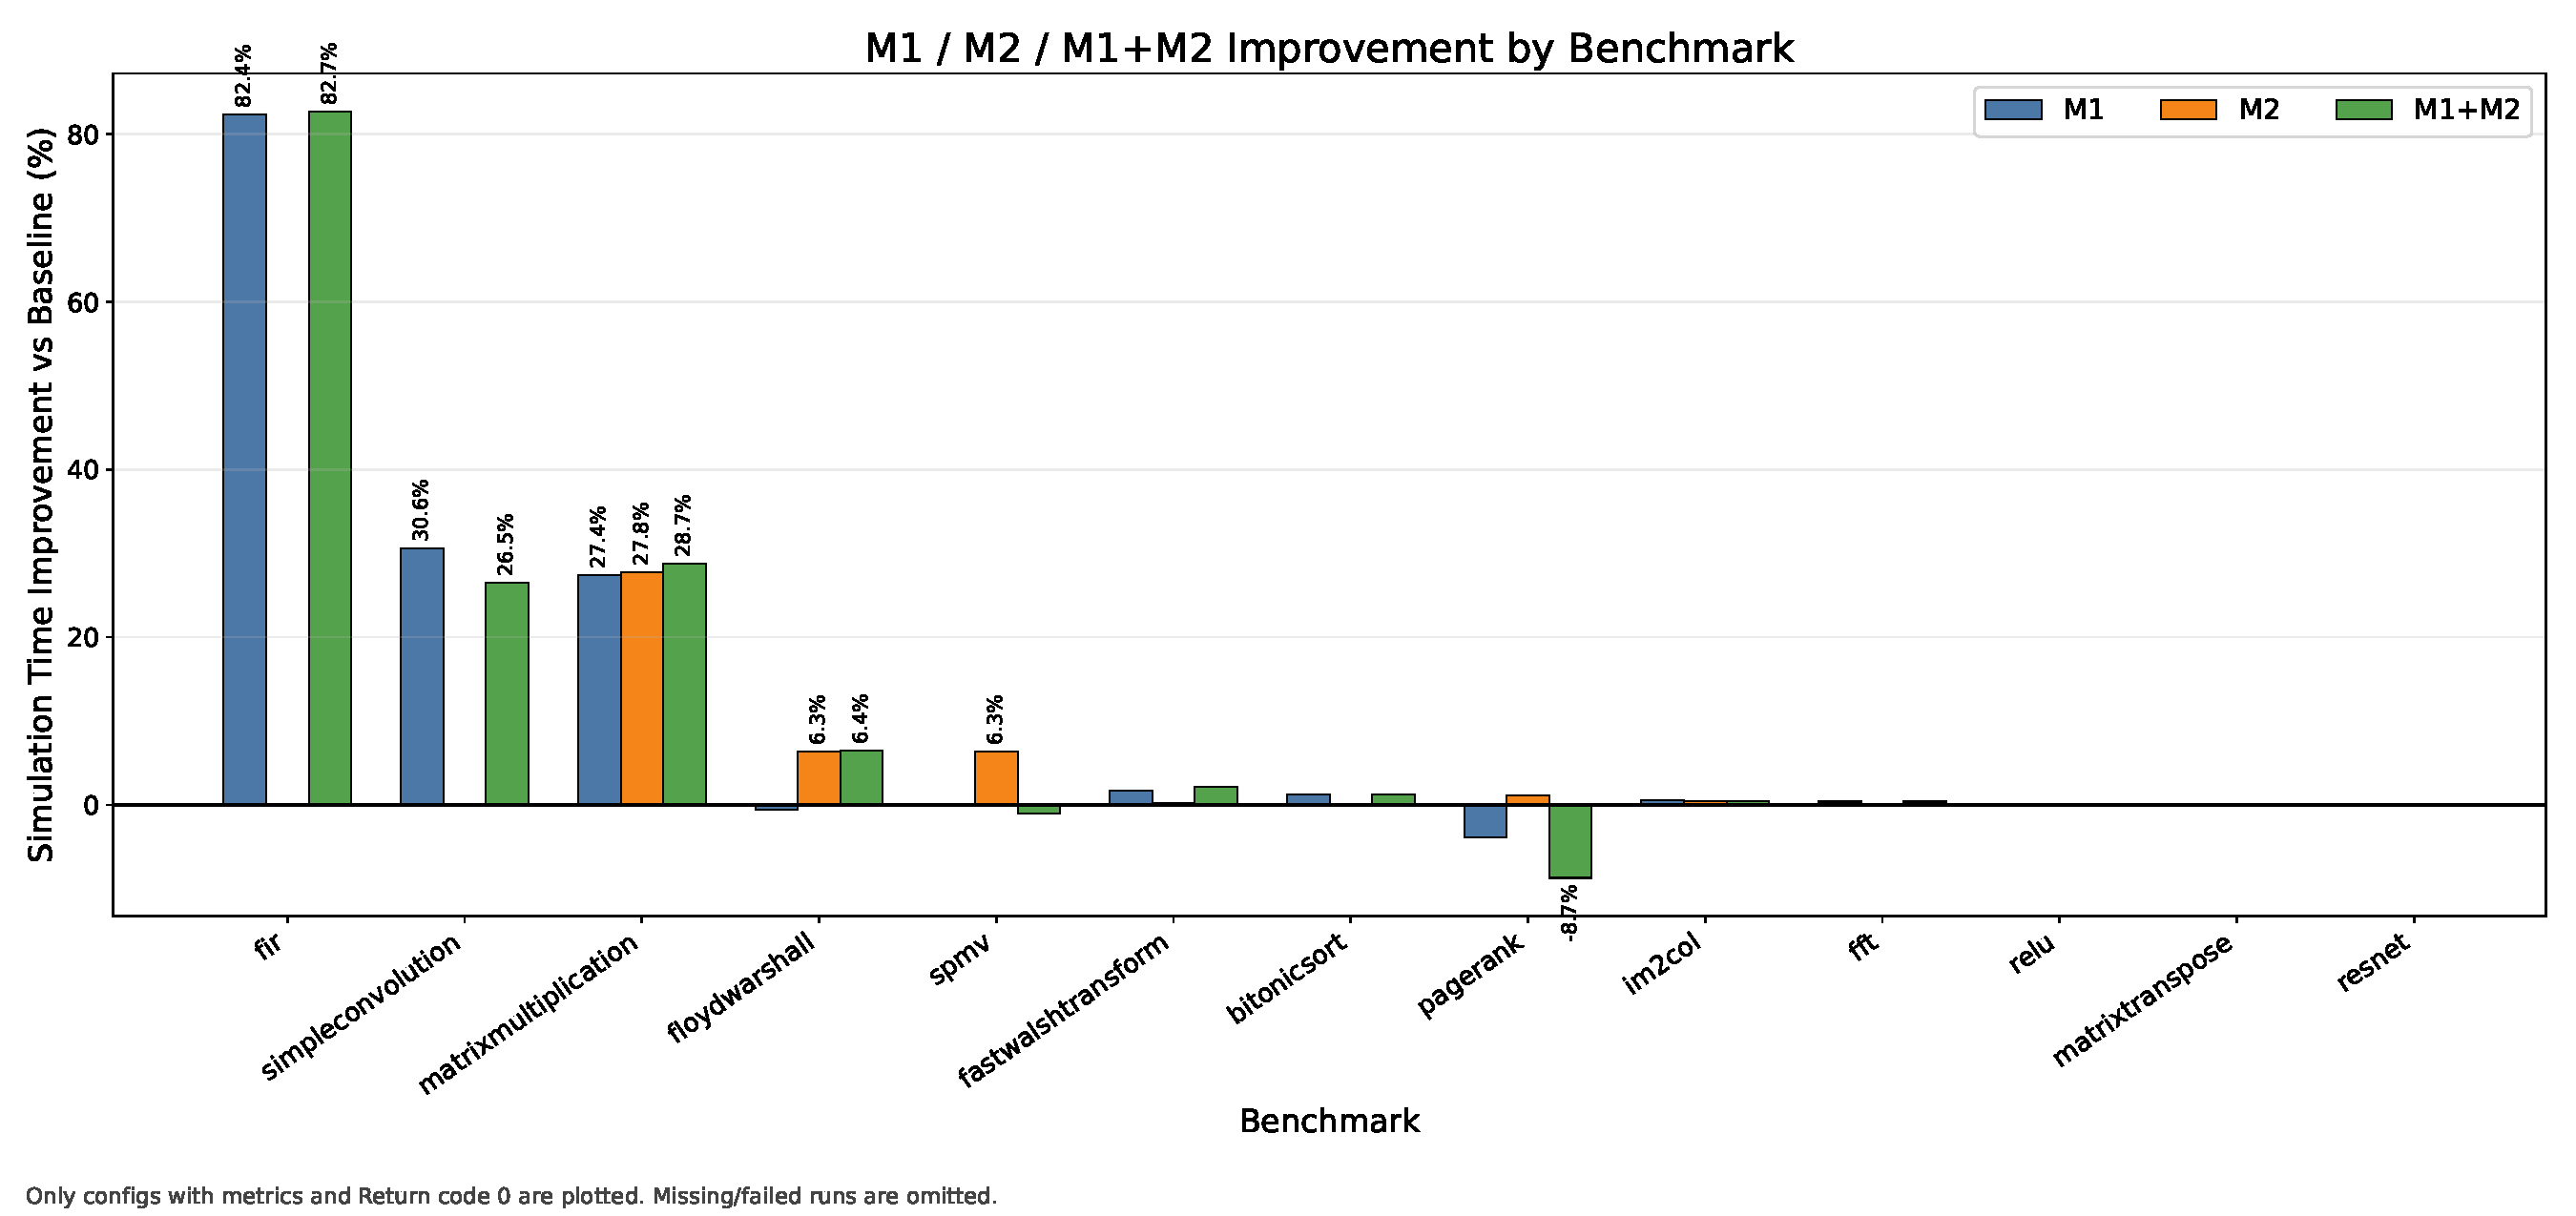
\includegraphics[width=0.95\textwidth]{figures/m1_m2_ablation_speedup.pdf}
  \caption{M1/M2 improvement from the June 29 all-mechanisms run.}
  \label{fig:simple-m1m2}
\end{figure*}

\section{Why Speedup Is Small}

M1 and M2 should be viewed as data-access datapath optimizations rather than
guaranteed end-to-end application optimizations.  As shown in
Figure~\ref{fig:simple-data-breakdown}, M1+M2 reduces the average cycles per
traced memory path for many workloads, which shows that the optimized datapath
is active and often faster.  However, the remaining latency can still be large:
remote-heavy workloads such as matrix transpose, PageRank, Im2Col, and SpMV
still spend hundreds of cycles per access in the network, while KMeans is
nearly unchanged.  Therefore, application speedup is small when the optimized
portion is not the dominant remaining bottleneck, or when the improved memory
path does not cover enough of the full execution time.

\begin{figure*}[t]
  \centering
  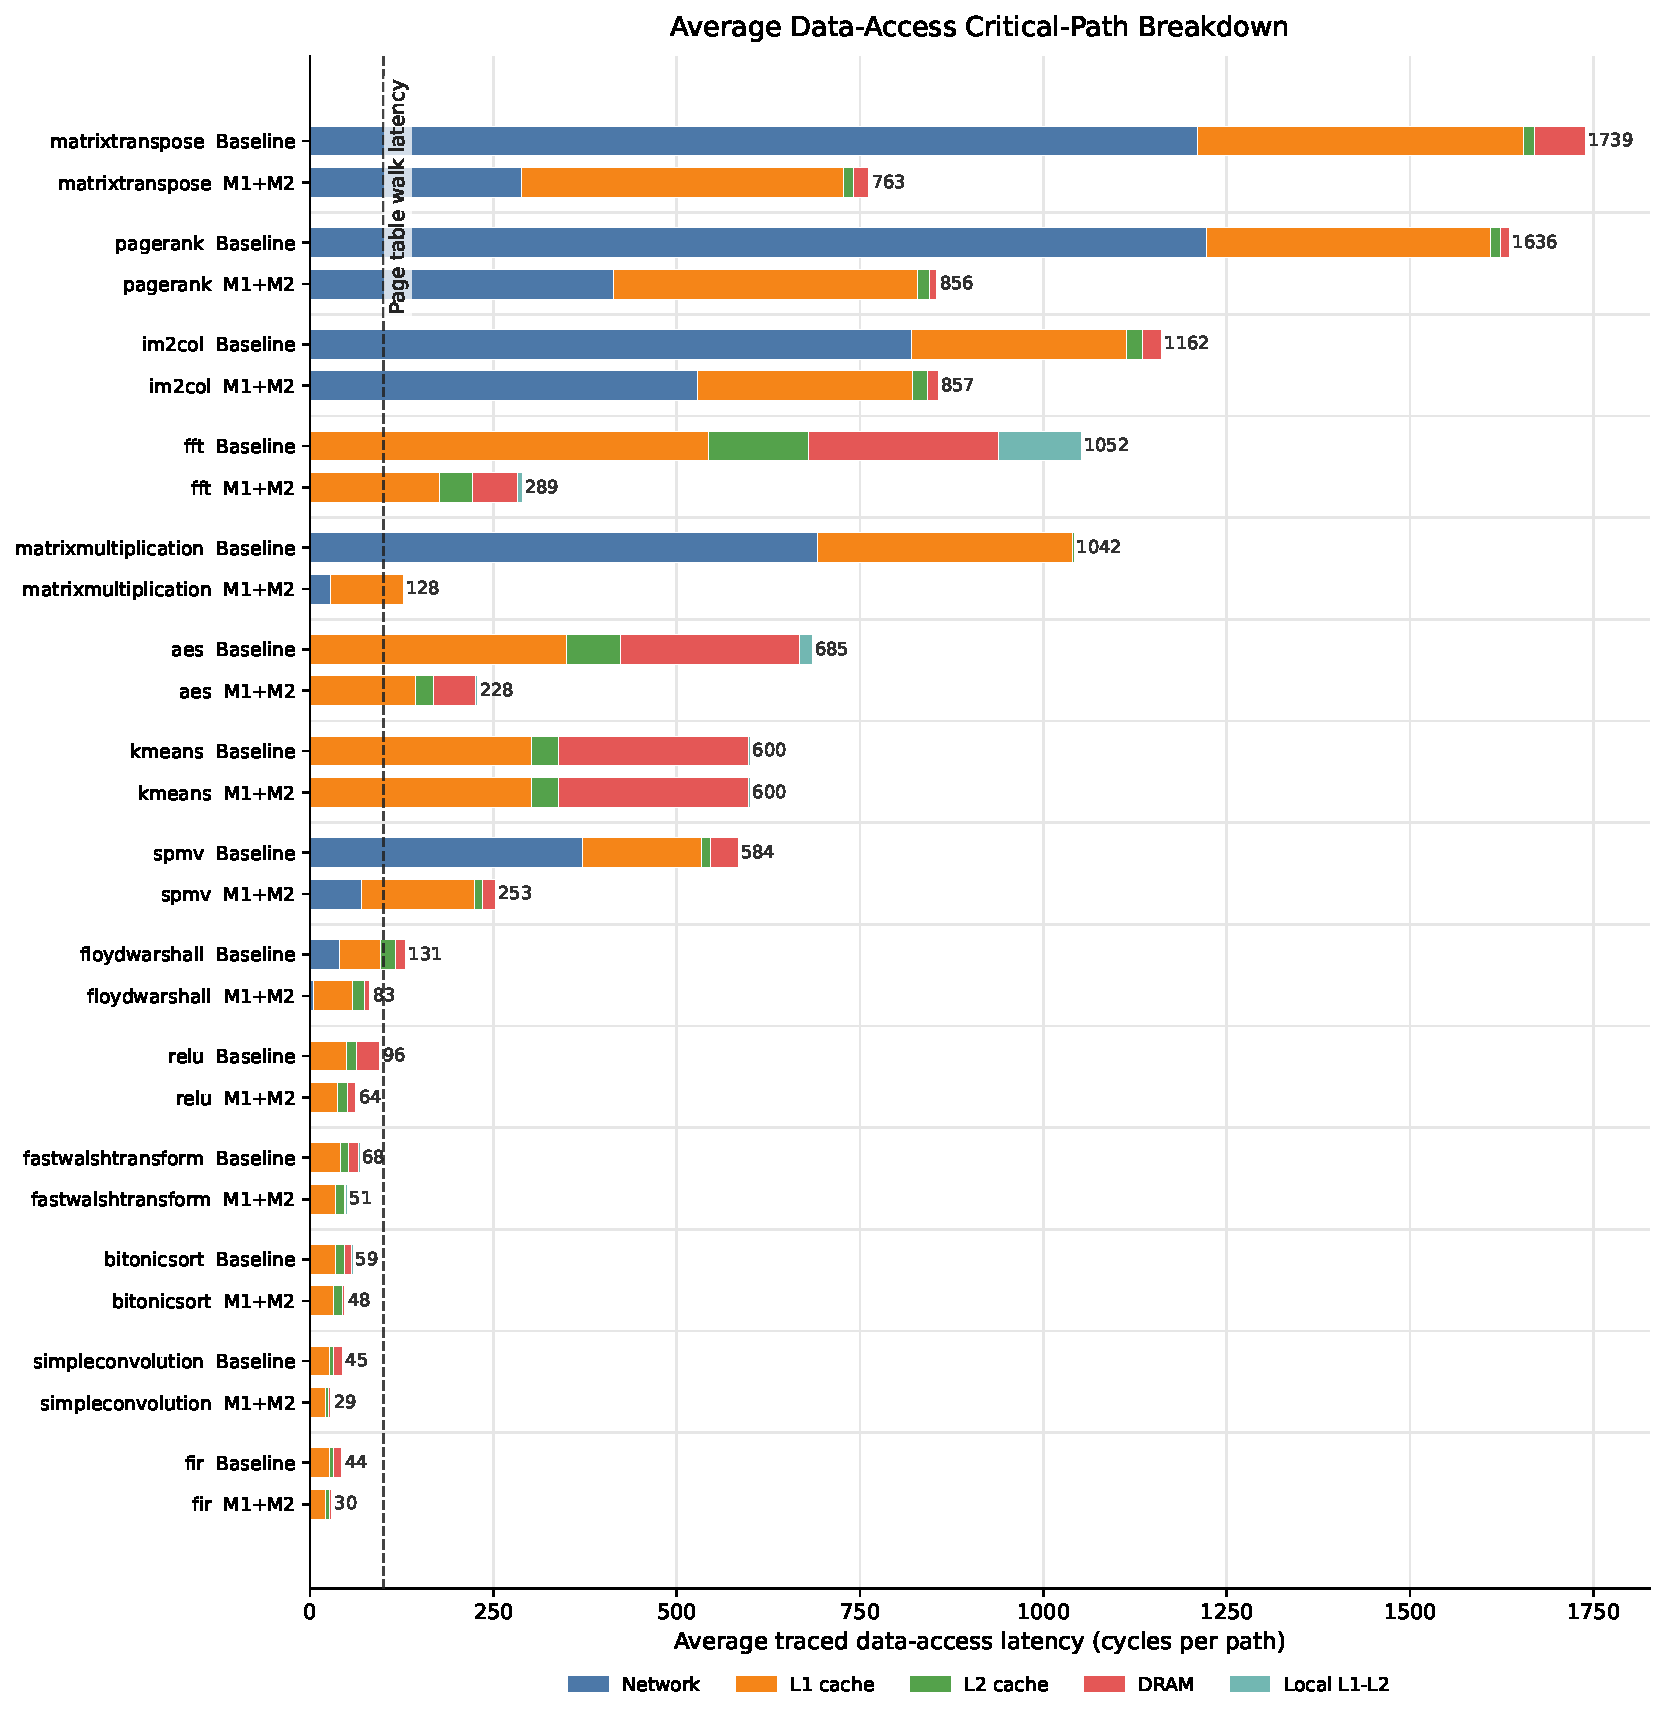
\includegraphics[width=0.95\textwidth]{figures/data_access_breakdown_avg_cycles_stacked.pdf}
  \caption{Average data-access critical-path breakdown for baseline and M1+M2.
  Values are traced latency cycles per memory path, split across network, L1
  cache, L2 cache, DRAM, local L1--L2 path, and other components.  The dashed
  vertical line marks a 100-cycle page table walk latency reference.}
  \label{fig:simple-data-breakdown}
\end{figure*}

\section{Remote-Network Motivation}

I added a remote-only streaming memory-path trace to record completed remote
L1V memory paths without keeping all raw records in RAM.  The baseline results
show that network/RDMA is the dominant part of the remote memory path in these
workloads.  Net. share is the fraction of remote memory-path latency spent in
network/RDMA, which ranges from 80.8\% to 95.6\% in the table.  GPU max/min is
the ratio between the largest and smallest requester-GPU average network
latency, showing that different GPUs can experience very different network
costs, up to 8.80$\times$ for KMeans.

\begin{table}[t]
  \centering
  \caption{Remote-only trace highlights.}
  \label{tab:simple-remote}
  \tiny
  \setlength{\tabcolsep}{3pt}
  \begin{tabular}{@{}lrr@{}}
    \toprule
    Workload & Net. share & GPU max/min \\
    & (\%) & \\
    \midrule
    SpMV & 92.7 & 4.20$\times$ \\
    MatrixTranspose & 80.8 & 1.61$\times$ \\
    PageRank & 95.6 & 2.21$\times$ \\
    MatrixMultiplication & 95.3 & 1.87$\times$ \\
    Im2Col & 86.2 & 4.03$\times$ \\
    KMeans & 87.2 & 8.80$\times$ \\
    FloydWarshall & 95.6 & 4.93$\times$ \\
    \bottomrule
  \end{tabular}
\end{table}

\begin{figure*}[t]
  \centering
  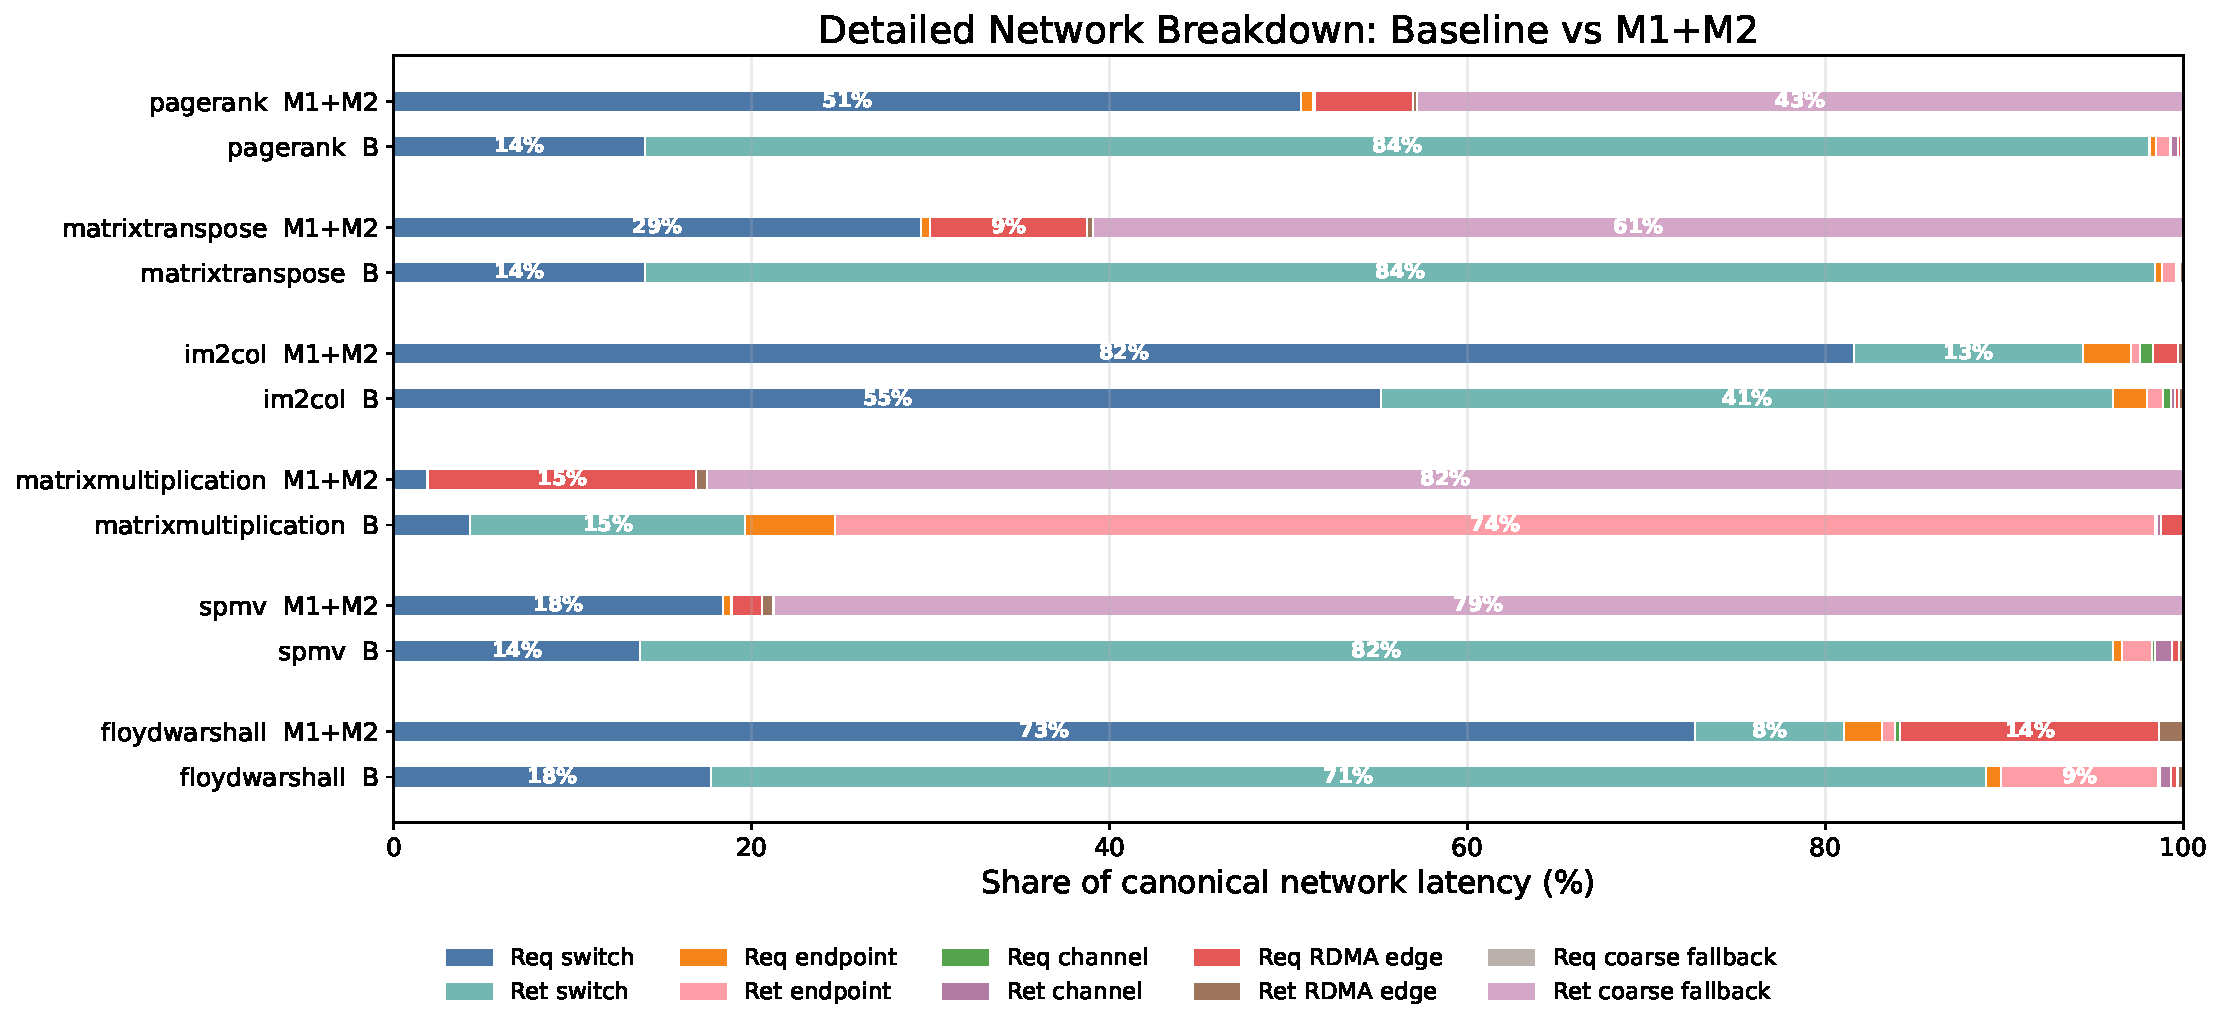
\includegraphics[width=0.95\textwidth]{figures/network_detail_percent_stacked.pdf}
  \caption{Detailed network breakdown for baseline and M1+M2.  Req is the
  request path from the requester GPU toward the remote owner; Ret is the
  response path back to the requester.  Req/Ret switch are NoC switch
  input-queue, pipeline, routing, arbitration, and output-wait cycles.  Req/Ret
  endpoint are endpoint queue, injection, assembly, and delivery cycles.
  Req/Ret channel are link-transfer cycles between endpoints/switches.  Req/Ret
  RDMA edge are cycles at the local/remote RDMA interfaces before entering or
  after leaving the network.  Req/Ret coarse fallback are aggregate RDMA-to-RDMA
  request/response stages used when fine-grained cross-GPU stages are not
  available.}
  \label{fig:simple-network-breakdown}
\end{figure*}

\begin{figure*}[t]
  \centering
  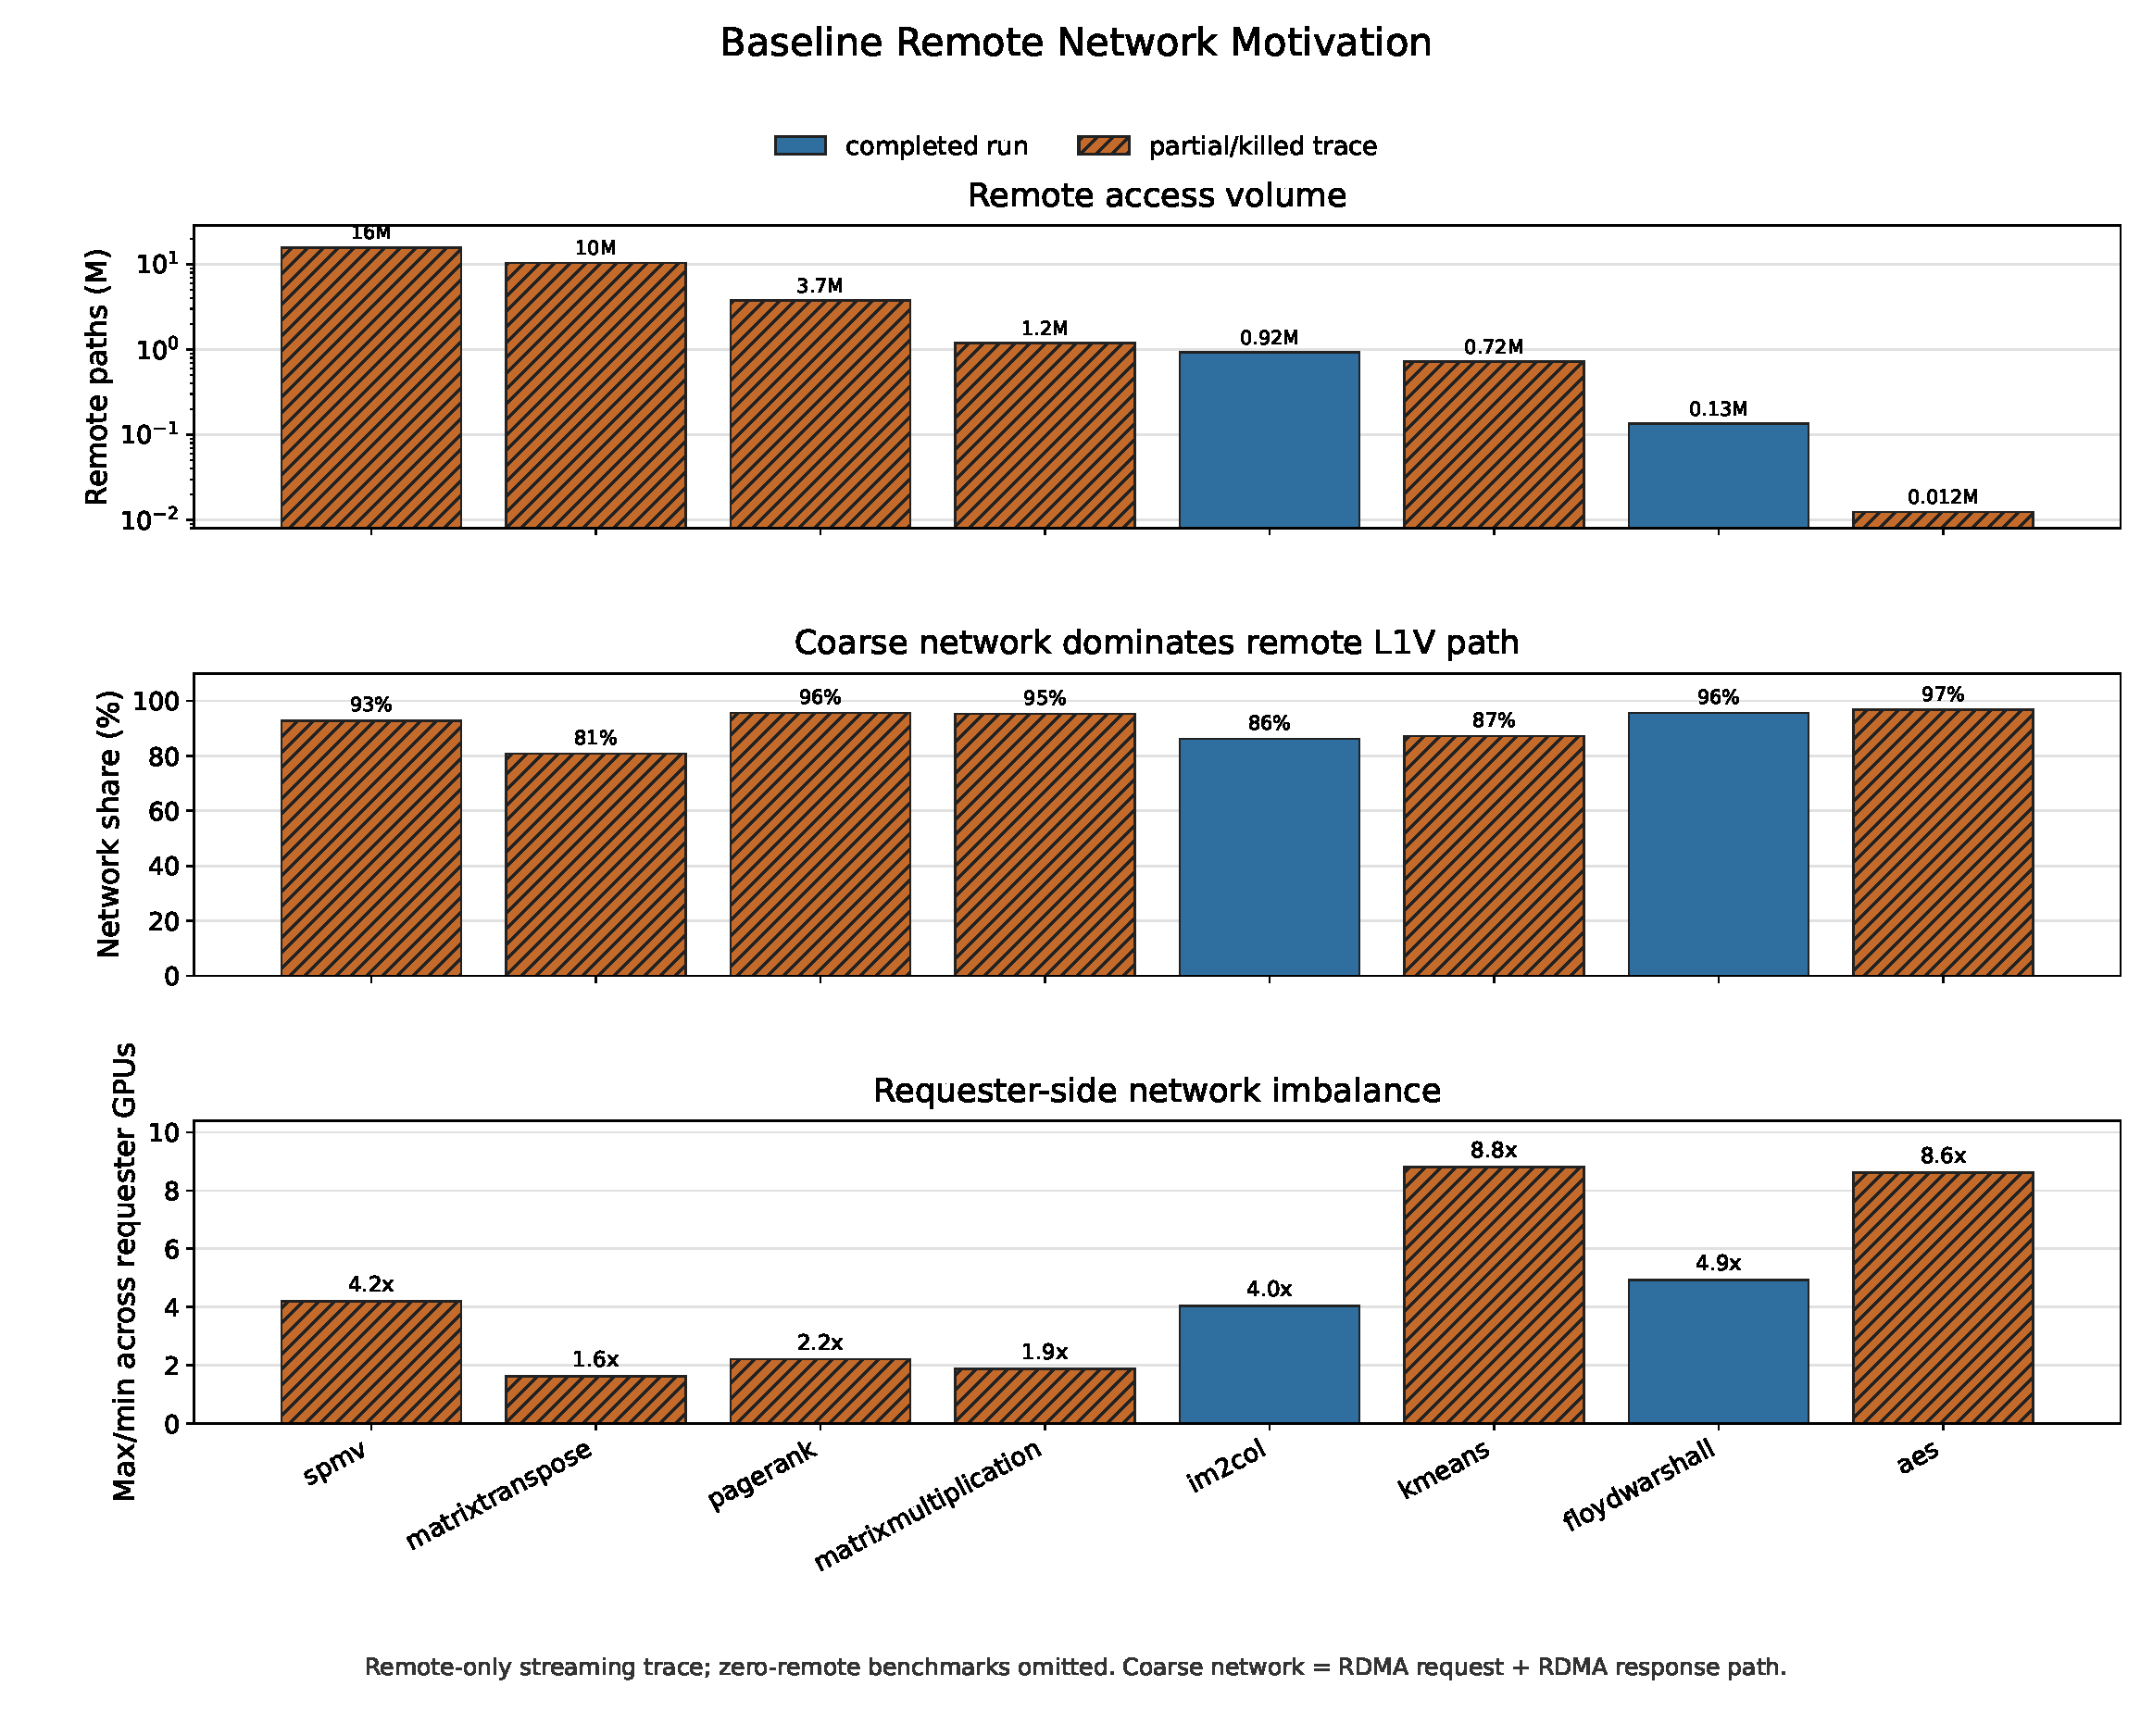
\includegraphics[width=0.95\textwidth]{figures/baseline_remote_network_motivation.pdf}
  \caption{Remote-network motivation from the baseline remote-only trace.}
  \label{fig:simple-remote}
\end{figure*}

\balance

\end{document}
